% !Mode:: "TeX:UTF-8"
% 文字编码:UTF-8
\chapter{引言}
\label{chap:intro}
随着带有摄像功能的便携智能设备的发展,以及各种无线网络覆盖率的提升,视频通话越来越多地应用在人们的日常生活中,如可视电话、视频会议、远程医疗、在线直播等。实时视频传输对网络质量要求较高,而目前无线信道存在的带宽波动、延迟、丢包等问题,使其面临很多困难和挑战。如何在多样化的网络环境下提供稳定和高质量的视频服务越来越成为工业界和学术界关注的热点。为此,本课题针对在无线网络上保障实时视频传输的质量,以及实现高可用性的视频通话系统进行研究。

\section{研究背景及意义}
人类通信的发展经历了飞鸽传书,邮寄信件,电报,固定电话,移动电话等阶段。在互联网出现后,又涌现出Email,网络语音,网络视频等更加方便快捷的通信形式,而移动互联网的发展更使人们随时随地都可以实现语音、视频通信。根据Cisco发布的全球移动数据预测报告\cite{index2016global},过去的2015年中全球移动网络数据流量增长了74\%,达到每个月3.7 艾字节,而到2020年这一数字预计将达到每个月30.6艾字节,人们对于移动互联网的依赖可见一斑。另一方面,如图\ref{fig:cisco_mobile}所示,2015年移动网络数据流量中,视频数据占比重为55\%,到2020年预计为75\%,以62\%的年均增长率成为移动网络中的绝对主流。可以想见,视频通话由于其实效性和丰富的信息量,必将成为人们日常通信的最主要方式。而无线网络作为便捷的网络接入方式,也将成为视频传输的最重要媒介。

与此相应的是,实时视频服务相关的产品和市场也蓬勃发展起来。日常通信方面,FaceTime、Skype、米聊等内置软件提供的视频聊天功能几乎成了智能手机系统的标配,而QQ、微信、环聊等社交软件也纷纷加入视频聊天功能,以此为基础的小游戏、互动软件也不断被开发出来。在企业全球化的今天,视频电话会议、远程医疗等也成为各大公司必备的生产力工具,具有极大的市场潜力。

近年来,电视盒子作为一种全新的互联网接入设备逐渐普及,使得电视机从单纯的电视节目播放转变成为家庭多媒体终端。除了观看网络视频以外,一些电视盒子还提供了视频通话功能,利用电视机高清大屏进行高质量的视频聊天。这一基于电视盒子的大屏视频通话,可以应用在日常通信、娱乐,视频会议,家庭监控等不同场景,具有较高的研究价值。当然电视盒子一般通过家庭Wifi接入互联网,视频聊天的效果也会受到无线网络一些不利因素的限制。
总之,越来越高清的视频质量和多样化的服务需求,给无线网络下的实时视频数据的高效传输提出了巨大挑战。

\begin{figure}[htbp]
  \centering
  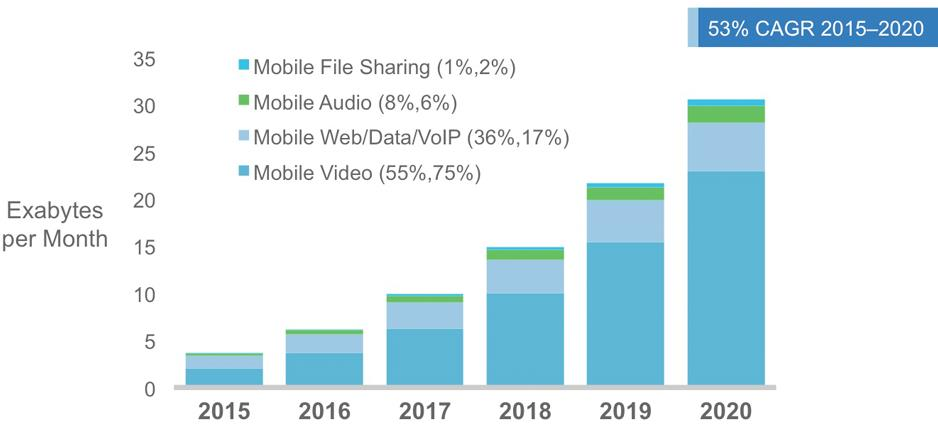
\includegraphics[scale=0.35]{cisco_mobile_traffic.jpg}
  \caption{2020年移动视频流量将占移动总流量的四分之三}
  \label{fig:cisco_mobile}
\end{figure}

高质量的视频通话体验依赖于较高的视频编码码率,较低的传输延迟,以及稳定可靠的传输信道。其中任何一项不满足,都会对用户体验造成很大的影响。而在网络传输方面,由于实时性的限制,基于重传的传统TCP协议并不适用于实时视频的传输,大部分实时视频传输都使用了面向数据包的UDP传输协议,在UDP协议层并没有对数据传输进行任何质量保障。无线网络信道的不稳定性,以及终端设备的多样化,也增加了实时视频的传输优化和质量保证的难度。具体来说,在无线网络中进行实时视频传输面临的主要问题包括:

\begin{itemize}
    \item 有限的网络带宽与越来越高的带宽需求之间的矛盾。视频数据信息量丰富,对网络带宽的需求也很大,过低的带宽会引起视频画面模糊、延迟增加,如果带宽低于视频最低压缩码率,则完全无法进行视频通话。同时为了保证通话过程中画面稳定,对带宽的波动也有一定限制。而无线网络由于终端位置移动、信号衰减等因素,带宽波动很大。
    \item 视频通话对延迟的高度敏感。由于视频通话涉及双方交互,轻微的延迟就会造成明显的通话不连贯。另一方面,为了保证视频播放连续性,每个视频包都需要在相应视频帧播放之前到达,否则就与丢包无异。而无线网络由于信道不稳定,本身存在一定的延迟。并且如果由于带宽波动引发网络拥塞,将产生更大的延迟。
    \item 网络丢包影响视频质量。由于视频文件编码特性,轻微的数据错误都可能造成连续画面的明显失真甚至无法解码。而无线网络下由于信号强度变化、终端移动等,发生数据错误和丢包概率大大增加。
\end{itemize}

针对以上实时视频传输和无线网络质量之间的一系列矛盾,视频码率自适应和非对称差错保护这两种技术可以在很大程度上对其进行改善,具体体现在:

\begin{itemize}
    \item 通过码率自适应算法及时合理地调整视频码率,可以保证网络负载始终稳定在网络承载能力以下,在实现较高带宽利用率的同时避免网络拥塞。既避免了网络拥塞引起延迟增大、丢包等影响视频传输质量的问题,又提高了视频平均码率。
    \item 对于信道不稳定造成的丢包,通过非对称差错保护添加冗余信息,可以为数据传输提供一定容错能力。使视频传输在高丢包环境下也能获得稳定的观看效果。
\end{itemize}

下面我们将介绍本文算法和系统中涉及到的一些基本概念。

\subsection{无线网络简介}
无线网络是指通过无线电波作为媒介进行传播的信息网络,一般我们提到的无线网络都与互联网相连,为用户提供移动互联网访问的能力。随着手机、笔记本电脑等移动智能设备数量激增,当今无线网络在技术、覆盖率等方面都有了极大的发展,其中蜂窝网络(如3G、4G)和无线局域网(WiFi)是目前应用最广泛的无线网络。无线网络具有架设快速、接入灵活、使用方便等优点,已经深入到人们生活的方方面面。本文关注的实时视频通信,其大部分应用场景都发生在手机蜂窝网络和家庭WiFi环境下。尽管如此,在无线网络的使用中仍然存在很多问题 \cite{heusse2003performance},包括:
\begin{itemize}
    \item 信号干扰:相比有线系统,无线网络经常受到电磁干扰,如其他无线网络或电磁设备等。这些干扰可能导致无线网络信号衰减、数据丢失等问题。
    \item 信号吸收和反射:无线信号在传播过程中会被某些材料吸收或反射,在覆盖范围内造成信号死角。
    \item 资源竞争:无线频谱是有限的资源,并由发射范围内的所有节点共享。如果多个无线网络出现频谱冲突,会造成网络带宽下降、延迟增加等问题。而随着无线网络需求增加,这一冲突的发生概率也越来越大。
\end{itemize}

在以上问题的背景下,无线网络下的视频传输需要解决带宽波动大、高丢包率、高延迟等问题,这对于视频通话系统的设计、算法优化都提出了特殊的要求。


\subsection{实时视频传输基本框架}

\begin{figure}[htbp]
  \centering
  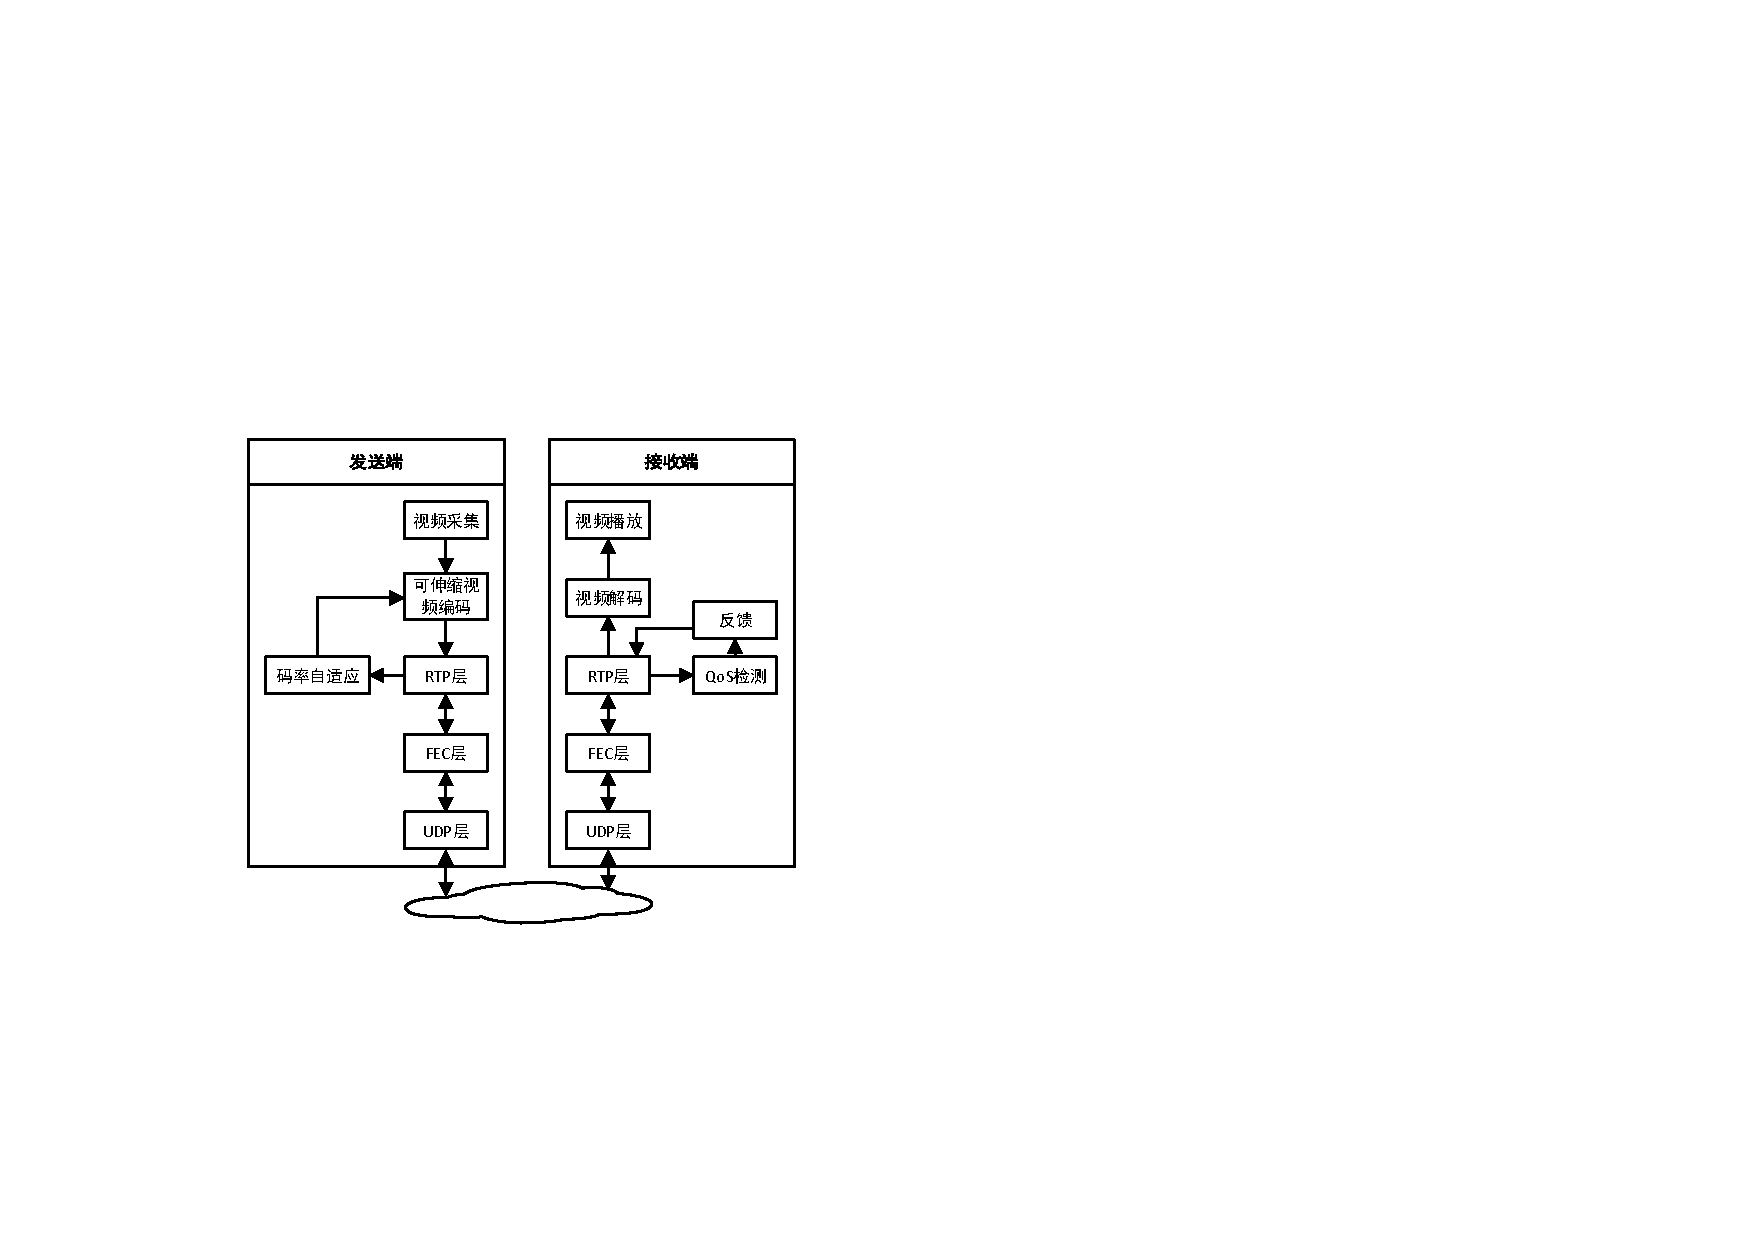
\includegraphics[width=0.7\textwidth]{steaming_architecture.pdf}
  \caption{实时视频传输基本框架图}
  \label{fig:steaming_architecture}
\end{figure}

尽管不同的实时视频通话应用实现方式千差万别,他们却有着基本相同的功能单元和整体架构,一个基本的实时视频传输系统框架如图 \ref{fig:steaming_architecture} \cite{wu2000transporting}所示。在发送端,视频采集模块通过摄像头等设备将自然场景转换为数字信号;可伸缩视频编码模块采用VP8、H.264等协议对原始视频信号进行压缩编码处理,生成码率可变的视频数据流;为了完成流式传输和观看,视频数据还需要在RTP层经过Real-time Transport Protocol(RTP)协议 \cite{jacobson2003rtp} 封装,添加序列号、时间戳等信息才能正确地在接收端实时解码和播放;为了应对丢包造成的失真,还可以在发送前对数据包进行FEC编码以添加冗余保护信息(可选);最后,数据由UDP层封装,通过更底层网络接口发送到接收端。这些数据包可能由于发生拥塞在网络链路上被丢弃,或由于超时而被接收端丢弃。接收端成功接收的数据包,经过一系列拆包、解码,还原为视频图像信息,并按照预定时间戳播放。

无线网络信号质量千差万别,其提供数据传输的能力也各不相同,这就要求通话双方根据网络状况合理选择发送视频的码率。为此,在实时视频传输系统框架中一般还加入了位于接收端的Quality of Service(QoS) 检测和反馈模块,用于检测当前通信信道的可用带宽、网络延迟、丢包率等信息;反馈模块将这些信息通过RTP协议附带的控制协议发送给接收端的码率自适应模块,在发送端根据不同的码率调整策略改变输出视频的码率,从而实现网络拥塞避免和网络带宽的有效利用。


\subsection{视频码率自适应}
在视频编码过程中,通过设定不同的分辨率、帧率、压缩倍数等,可以动态改变输出视频数据流的码率。例如在较差的网络条件下使用较低的视频码率,虽然损失了一定的画面清晰度,但是由于带宽需求更低,至少能够保证通话过程的平滑流畅。而在带宽充足的情况下,使用较高的视频码率可以充分利用带宽,提供更清晰的视频画面。利用这一思路,通过在通话过程中不断调整视频码率,可以在保证通话顺利进行的前提下,尽可能提高网络带宽利用率,从而获得更好的视频体验。然而这一调节过程本身存在矛盾:如果过分强调带宽利用率,采取激进的码率策略,一旦网络出现波动很容易造成拥塞;而过于保守的码率策略则会造成带宽浪费。因此如何根据网络状况准确调节视频码率,是进行视频传输需要重点解决的问题。

另一方面,实时视频作为一种实时流媒体,与一般网络数据传输最大的不同就是它对数据实时性的要求,一旦数据到达时间超过了有效播放时间,则与丢包无异。而网络上应用最广泛的 TCP 传输协议通过维护拥塞窗口以及丢包重传机制保障数据传输的可靠性,却也因此引入了较大的传输延迟,并不适用于网络上比重越来越大的实时流媒体传输。这就要求我们为实时视频传输设计专门的码率自适应算法。

\subsection{视频传输的非对称差错保护}
实时视频传输和普通文件传输的一个重要区别就是,视频数据即使发生了部分错误,仍然可以继续播放,只是部分画面会出现马赛克或丢帧,降低一定的用户体验。因此在很多视频通话应用中,差错控制模块都属于可选模块。但如果视频传输在高丢包率的无线网络条件下进行,过多的丢包就会对视频质量造成严重影响,需要通过一定的差错控制措施来减少丢包造成的质量损失。最常用的实时视频传输差错保护方法就是FEC冗余编码,通过向发送数据流中加入冗余信息提供一定纠错能力,在接收端即使只收到部分数据,仍然有可能解码出原始信息。

由于视频编码过程中进行了数据压缩,一个视频流中不同的数据重要性一般是各不相同的。有些数据一旦丢失会造成多个视频帧无法解码,而有些数据只会造成某一帧画面上的少量失真。一种直观的想法是在FEC冗余编码过程中重点保护那些更重要的数据,为它们分配更多的冗余信息。这种根据数据重要程度不同进行不同程度保护的策略成为非对称差错保护。而冗余信息分配是否合理,也在很大程度上影响了冗余保护的效果。因此研究视频传输的非对称差错保护,是提升视频通话质量的一种有效途径。

另外,在FEC编解码过程中,单个编码块的大小(即一次编码所包含的数据包数量)对于编解码效果有很大影响。编解码单元越大,FEC编解码效率越高,灵活性也越好。然而如果采用较大的编解码单元,在发送端需要等待编码块中数据包涉及到的视频帧全部编码完毕才能进行FEC 编码,接收端则需要等待编码块中所有数据包接收完毕才能实现FEC解码,这都会引入额外的编解码延迟,从而对延迟敏感的实时视频传输产生较大影响。因此如何在不引入额外延迟的前提下提升FEC编解码效率也是实现差错保护过程中需要关注的问题。

\section{研究内容}
\begin{figure}[htbp]
  \centering
  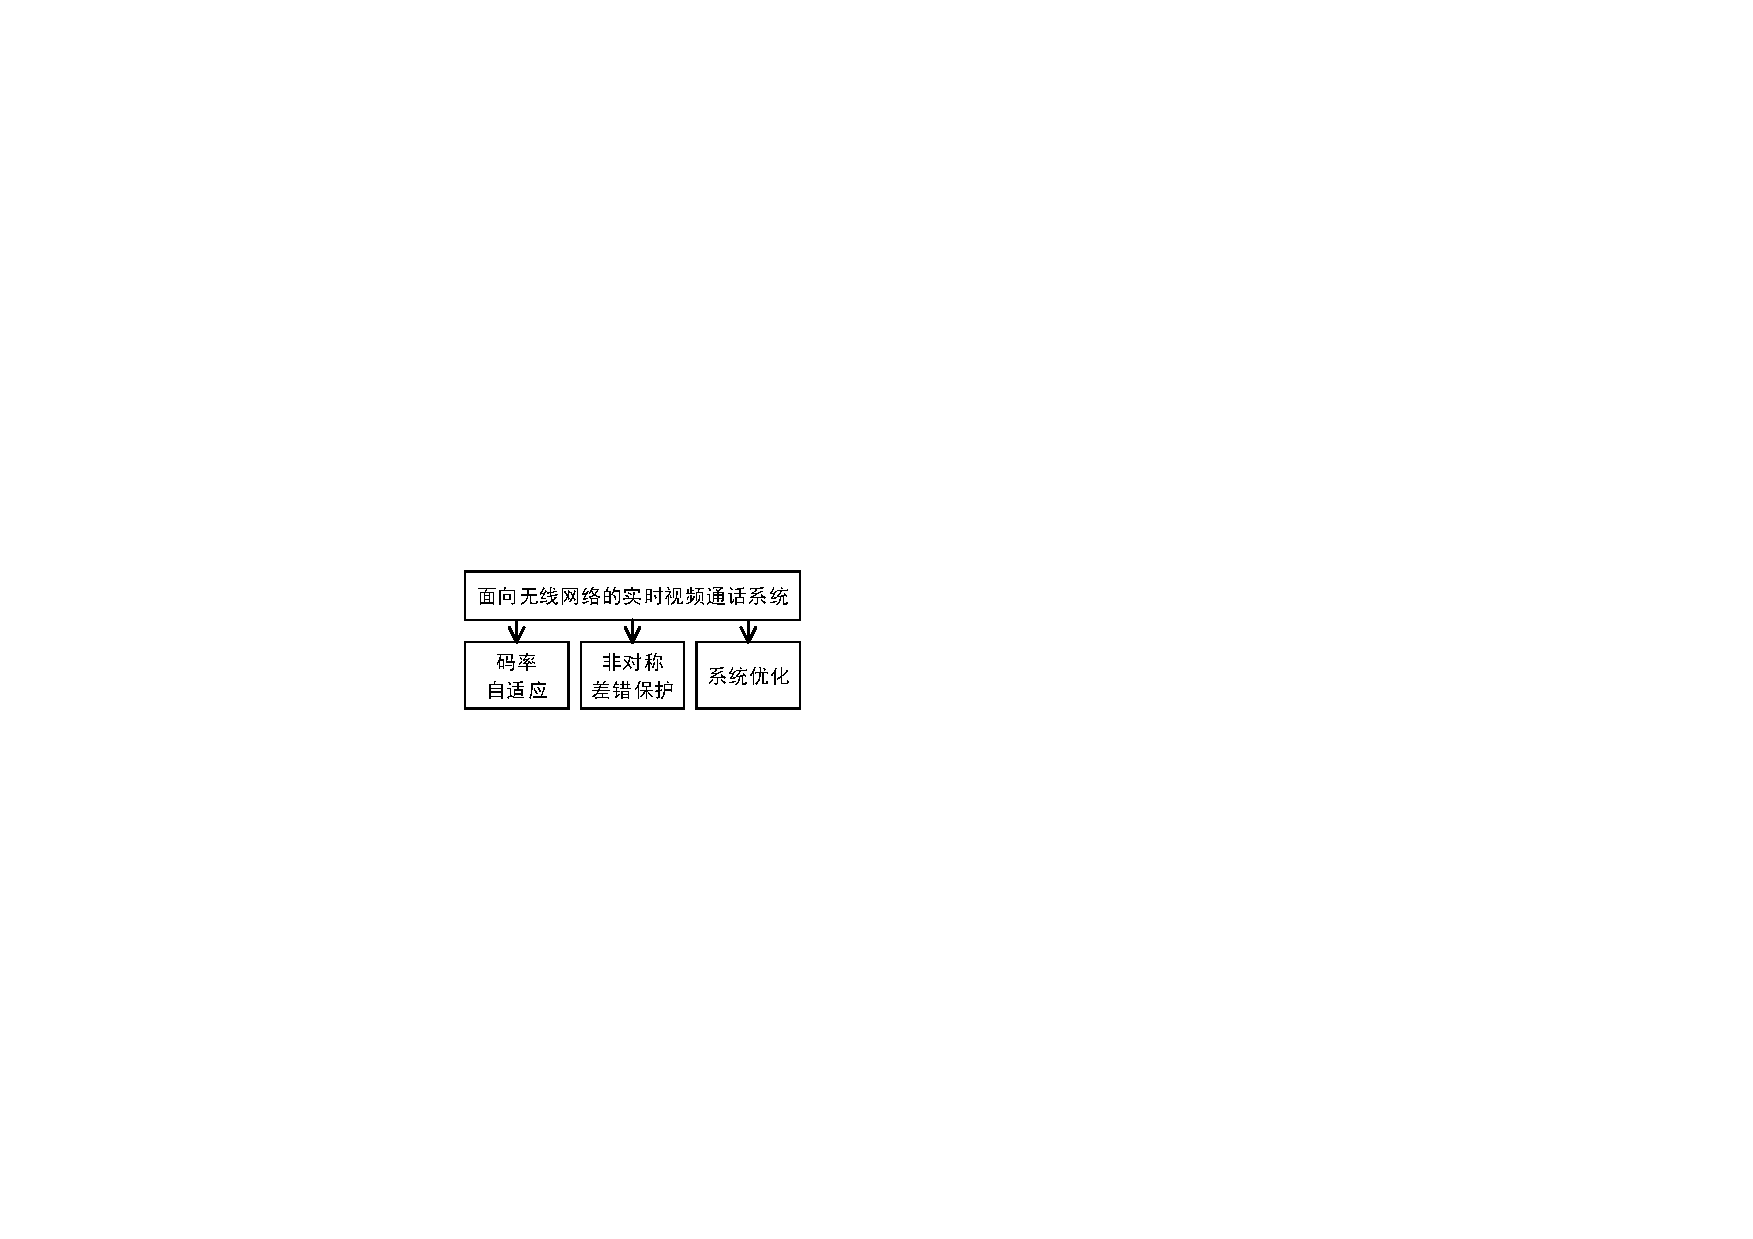
\includegraphics[width=0.5\textwidth]{research_architecture2.pdf}
  \caption{研究框架}
  \label{fig:research_architecture}
\end{figure}

基于上述背景,我们希望实现一个能够在无线网络中提供高质量服务的实时视频通话应用,同时结合电视盒子大屏幕的特性提供高清视频通话服务。我们以图 \ref{fig:steaming_architecture}中的实时视频传输基本框架为原型,基于开源VoIP软件Linphone搭建了面向电视盒子的实时视频传输原型系统。
该系统中对通话质量影响最大的就是复杂网络状况下视频码率的确定,以及高丢包环境下如何保证视频解码成功率。

针对上述问题,我们以图 \ref{fig:research_architecture}为研究框架,在以下几个方面展开研究:
首先,为了在网络带宽不稳定、丢包和延迟都更加严重的无线网络下实现稳定的视频传输,我们提出一种基于排队延迟的码率自适应框架,实现延迟可控的视频传输,并用控制论模型对调整过程进行优化;
然后,为了减小无线网络高丢包率对视频质量的影响,我们引入了非对称差错保护模块,并对非对称差错保护算法中的冗余分配这一关键环节进行了优化;
最后,综合上述算法,我们对视频通话系统的实现细节进行了优化,对界面进行改进,以提高大屏幕电视界面下的视频通话质量和用户交互体验。

\subsection{延迟优化的实时视频码率自适应算法}
高质量的实时视频传输服务要求较大且稳定的带宽、低延迟和低丢包率等,这对于网络拥塞控制也就是视频的码率自适应算法提出了很高的要求。而大部分现有拥塞控制算法主要着眼于避免网络拥塞和整体流量的公平,单个数据流获取到的带宽和网络延迟往往存在很大的波动,这极大降低了实时视频的用户体验。
尤其是在无线网络的背景下,没有进行过专门优化的码率自适应算法往往无法适应高丢包率的环境,存在带宽低估、延迟过大等问题。

本研究通过排队延迟模型对网络进行建模,分析排队延迟变化与视频码率之间的关系,进而以网络延迟为反馈信号动态调整视频码率。
另外通过引入控制论模型和PID控制器对码率调整过程进行优化,合理权衡系统稳定性和响应速度,进一步提高了码率自适应的效果。
大量实验结果表明,该码率自适应算法在带宽利用率和码率稳定性方面的表现均超过了已有主流方法,同时在传输过程中保持了较低的网络延迟,特别适用于实时流媒体的传输。
相关研究成果已发表于IEEE VCIP-2015。

\subsection{基于非对称差错保护的冗余分配优化算法}
基于扩展窗口的FEC技术具有不引入额外延迟,控制失真扩散等特点,特别适合无线网络上的实时视频传输。具体来说,考虑到视频数据的非对称特性,我们可以对差错保护效果与冗余分布的关系进行数学建模,求解最优的冗余信息分配策略,来优化差错保护的效果。而由于扩展窗口的引入,这一优化问题变得层层嵌套,十分复杂,直接求解的难度很大。

本文针对扩展窗口FEC框架中冗余数据的分配问题进行研究,提出一种基于此框架的冗余分配方案。我们首先针对扩展窗口编解码的数据包进行等效丢包率分析,并针对其编解码特征提出了关于数据包解码条件的两条推论。然后我们推导出了GOP整体语预期失真公式,作为冗余最优化分配的理论基础。在此基础上,冗余分配问题被归纳为带约束的非线性优化问题,并用简化了复杂度的贪心算法进行求解。大量实验结果表明,应用本算法得到的冗余分配策略进行扩展窗口FEC冗余保护,在各种网络场景下都能明显提高视频传输的FEC 保护效果。相关研究成果已经发表于IEEE ICIP-2015。

\subsection{面向电视盒子的实时视频通话系统}
在上述算法研究的基础上,我们以一个开源VOIP软件为基础,对其底层码率自适应模块进行重写并添加FEC差错保护模块,同时重写用户交互界面,实现了一个面向电视盒子的视频通话软件。首先在底层RTP 和RTCP 协议的基础上实现了一个码率自适应模块,以当前网络的延迟和丢包信息为输入,根据本文提出的码率自适应算法实时调整视频码率。另外,我们还实现了一个独立的差错保护模块,对底层RTP 包进行基于扩展窗口框架的FEC冗余编码和解码,在网络丢包时对视频数据进行恢复,从而更好地适应高丢包率的无线网络环境。最后,考虑到电视盒子的普及和未来视频通话的发展趋势,我们还将这一系统移植到电视盒子上,为家庭用户提供更加高质量的大屏视频通话体验。

\section{论文结构}
本论文的结构安排如下。
第 \ref{chap:intro}章首先介绍了论文的研究背景和意义,以及相关领域面对的挑战。
第 \ref{chap:related}章介绍了实时视频码率自适应和视频流差错保护方面的国内外研究现状。
第 \ref{chap:rate}章以现有拥塞控制算法为基础,考虑实时视频服务对延迟的需求,提出了一种延迟优化的码率自适应算法。
第 \ref{chap:fec}章考虑在易丢包的无线网络下进行视频传输的需求,提出一种视频流非对称差错保护中的冗余分配算法。
综合以上两种算法,我们在第 \ref{chap:system}章设计了一个面向电视盒子的高清视频通话系统。
最后在第 \ref{chap:conclusion}章对本文进行总结和未来工作的展望。
